\subsection{Applying Material Feature Manipulations}
\label{sec:dataset-material-feature}
The objective is to clone every model and apply a color feature to every clone to be able to distinguish the same models.
Cloning is a trivial task because this can be done by rendering the native object first and then the color featured one.
One method for the color feature manipulation is preparing a color feature like a colored circle as an image and putting it on the model.
This feature can be scaled dependently on all the face areas for achieving a similar scale across all models.
However, clinging this image to a model considering all its edges is problematic.
It would be necessary to find a way to unfold the model along its edges.
This can be done by hand but is very time-consuming and complex.
In fact, Blender supports an automatic way of unfolding, but its results are not satisfying.
Therefore, this approach is not further pursued.
Another method is to color vertices.
However, for achieving reasonable features, a high number of vertices is necessary.
There is an option to subdivide existing faces and add additional vertices, but this increases the data size extremely, which needs much more computer performance and has the risk of inducing unwanted geometry into the model.
Hence, coloring single faces becomes the chosen approach due to its simplicity.
In CAD modeling objects are assigned a material with a color that reacts to light which produces shadows.
In Blender, the default material's color is a slightly darkened white.
Changing the color of a face is performed by changing the color of its material.

For following this approach, it is advisable to pre-define material presets.
Those presets consist of the default material but have different colors.
After making those presets available to the Blender scene, a well-suited face for being colored needs to be found.
In the following those faces are referred to as an optimal face.
It is important to filter all faces of an object by their area size.
\figref{fig:face-area-filter} shows why and the results of several thresholds.
\begin{figure}
	\centering
	\begin{subfigure}{.32\textwidth}
		\centering
		
\includegraphics[width=\textwidth]{images/face_area_unfiltered.png}
		\caption{Unfiltered}
		\label{fig:face-area-unfiltered}
	\end{subfigure}
	\begin{subfigure}{.32\textwidth}
		\centering
		
\includegraphics[width=\textwidth]{images/face_area_mean.png}
		\caption{Face Area Mean}
		\label{fig:face-area-mean}
	\end{subfigure}
	\begin{subfigure}{.32\textwidth}
		\centering
		
\includegraphics[width=\textwidth]{images/face_area_max_dependent.png}
		\caption{Max Face Area Dependent}
		\label{fig:face-area-max-dependent}
	\end{subfigure}
	\caption{Threshold setup for filtering faces by their area size}
	\label{fig:face-area-filter}
\end{figure}
If faces are not filtered at all, any face can result in being the optimal one.
However, it is not guaranteed that this face has a decent size and can be seen and recognized by the network easily.
This assumption was later verified by a not changing loss value during training.
Like in \figref{fig:face-area-unfiltered} the optimal face is comparatively small to the whole model.
Accepting only faces as the optimal face, that have at least the size of the mean of all faces lead to a result like in \figref{fig:face-area-mean}.
The optimal face can be seen more easily than before, but this threshold often results in long and slender optimal faces.
This is due to the fact, that the chosen object categories mostly contain objects that are built using such faces because they have longish surfaces.
Hence, filtering by the mean of the faces amplifies the probability to choose such a face as an optimal one.
Therefore, a threshold of above the mean is desired to skip all those lathy faces like it is shown in \figref{fig:face-area-max-dependent}.
Additionally, larger faces should be preferred.
Thus, the area of the optimal face have to satisfy
\begin{equation}
	a_{opt} > (a_{mean} + a_{max}) \cdot s
\end{equation}
where $a$ are the related areas and $s$ a scalar.
With $s = 0.3$ satisfying results are achieved.

Furthermore, it needs to be guaranteed, that the optimal face is visible in at least one view and not visible in at least one view.
This is validated by casting rays from the camera center onto the possible optimal face for every camera position that was defined in \secref{sec:dataset-rendering}.
In brief, if the rays hit the face, the face is visible.
Fortunately, there is a function in Blender performing this approach and returning among others the index of the face that is hit.
However, this cannot be performed for every pixel of a face due to performance issues.
Thus, the trade-off against accuracy is only checking the vertices defining the face.
This can raise errors, though, because a vertex can define multiple faces and it is not certain which face index the function returns.
Hence, each checkpoint $\vec{p}_i$ is moved slightly to the center of the face by
\begin{equation}
	\vec{p}_i = \vec{v}_i + 0.05 \cdot (\vec{f}_0 - \vec{v}_i)
\end{equation}
where $\vec{v}_i$ is the related vertex and $\vec{f}_0$ the center of the face.
If the ray cast is valid for at least one checkpoint the face is supposed to be visible.
If all rays hit the wrong face, the current face is supposed to be not visible.
As soon as both conditions are satisfied for the examined face among all views, it becomes the optimal face.
Otherwise, the next possible face is investigated.
If the conditions are never satisfied for each possible face, the object is skipped at all.

It is found, that a single optimal face is not enough, because some models have several duplicated faces.
Those are different faces where the coordinates of all the describing vertices are identical to the ones of other faces.
Hence, there are faces laying into each other.
This results in rendering issues like it is shown in \figref{fig:optimal-face}, because the rendering engine does not know, which material should be rendered on the surface.
In \figref{fig:optimal-face-single} only one of two identical faces is colored, which leads to the noticeable transparency effect.
That is one of the brighter effects, though.
It is also possible that one optimal face is shown normally and only on the edge rendering issues are visible like a dotted line with the colors of all optimal faces. 
Nevertheless, any of these effects could induce false correlations into the dataset that are not available on real-world objects, hence, leading to a not practical network.
Thus, in \figref{fig:optimal-face-all} the materials of all identical faces are changed, which leads to realistic color representations.
\begin{figure}
	\centering
	\begin{subfigure}{.49\textwidth}
		\centering
		
\includegraphics[width=.7\textwidth]{images/optimal_face_single.png}
		\caption{Single Optimal Face}
		\label{fig:optimal-face-single}
	\end{subfigure}
	\begin{subfigure}{.49\textwidth}
		\centering
		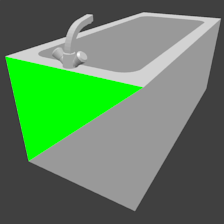
\includegraphics[width=.7\textwidth]{images/optimal_face_all.png}
		\caption{All Optimal Faces}
		\label{fig:optimal-face-all}
	\end{subfigure}
	\caption{Material manipulation on duplicated optimal faces}
	\label{fig:optimal-face}
\end{figure}

Regarding a validation of the later model, an examination of two material features per object would be interesting.
Hence, for applying another material change on a model, another optimal face or faces, respectively, needs to be found.
A requirement for this is the presence of only one material feature in a single view.
Due to the automation of this task, a reliable solution is necessary.
One approach would be using the other side of the surface of the first optimal face.
However, this fails if the surface has a thickness of more than a single face.
Then the next face along its normal needs to be found by ray casting and then the visibility of this face needs to be verified.
Thus, this process leads to excessive ray cast validations and therefore not followed up on.
However, it is considered, that faces at a similar location as the original optimal face are well-suited as well.
Thus, the choices of further optimal faces are narrowed down by sorting all remaining faces by their distance from their center to the center of the first optimal face in descending order.
The intention is that choosing faces with the largest distances result in either a kind of opposite face or in a face that is that far away to not be visible at the same time. as the first optimal face.
Of course, the tasks of checking the visibility and finding identical faces are performed on the new face as well.
If no additional optimal face is found, the model is skipped, although, this never happened during execution.